\documentclass{multi}

\title{Polar, spherical, cylindrical coordinates, coordinate transforms}
\course{Math 60: Multivariable Calculus}
\date{Monday, 25 September 2017}

\begin{document}

\paragraph{Example}

Consider the integral
\[
    \int_0^2 \int_{y^2}^{4} y \cos (x^2) \, \diff x \, \diff y.
\]
If we directly try to evaluate the integral, we run into the problem that \(\cos (x^2)\) \emph{cannot be integrated}! That's not good. But let's try to ``visualize'' the integral:
\begin{center}
    \begin{tikzpicture}

\tikzstyle{ax} = [thick, -stealth];

\draw[ax]
    (-1,0) -- (4,0)
    node[right]{\(x\)};

\draw[ax]
    (0,-1) -- (0,3)
    node[above] {\(y\)};





% signed volume

    \end{tikzpicture}
\end{center}

\section*{Polar coordinates}

\paragraph{Example}
 
\newcommand{\pie}{
    \fill[lightgray]
        (0,0) -- (2,0)
        arc[radius=2, start angle=0, end angle=-300]
        -- cycle;
    
    
    \draw
        (0,0) 
        circle[radius=2];
    
    \draw
        (2,0) -- (0,0) -- (-300:2);
}

Say we want to find the area of some region \(R\) in a circle: % arc section
\begin{center}
       
    \begin{tikzpicture}

\pie

\path
    (-150:1) node {\(R\)};

    \end{tikzpicture}
\end{center}
There are two ``obvious'' ways to ``parametrize'' this integral (recall that integration can be thought of as cutting the area into thin, infinitesimal slices, and then ``summing'' some function over the infinitely many tiny slices):
\begin{itemize}
\item In \emph{cartesian} (\(x\) and \(y\)) coordinates:
    \begin{center}
        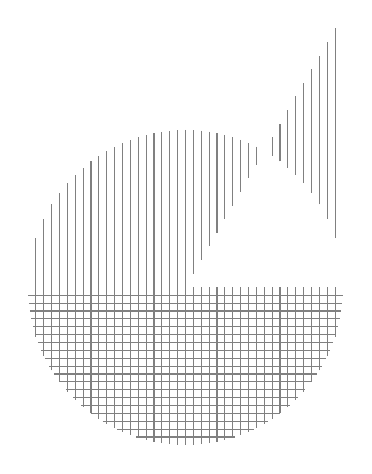
\begin{tikzpicture}
            
\pie

\foreach \i in {1,...,19} {
    \draw[black!50]
        ({-\i/10},{-sqrt(4-(\i/10)^2)}) -- ({-\i/10},{sqrt(4-(\i/10)^2)})
        ({-sqrt(4-(\i/10)^2)},{-\i/10}) -- ({sqrt(4-(\i/10)^2)},{-\i/10});
}
\foreach \i in {0,...,19} {
    \draw[black!50]
        ({\i/10},{-sqrt(4-(\i/10)^2)}) -- ({\i/10},0)
        ({\i/10},{sqrt(4-(\i/10)^2)}) -- ({\i/10},{\i/10*tan(60)});
}
        \end{tikzpicture}
    \end{center}
\end{itemize}

\section*{Triple integrals}

Picture 
% gold density integration over mass of gold


% summing over inner cubic slices/pieces of region
% visualization: projection onto xy-plane, integration inside a "pole"

\paragraph{Example}

Consider the volume inside the capsule bounded by the paraboloids \(z = 9 - x^2 - y^2\) and \(z = 3x^2 + 3y^2 - 16\). 

% visualization of thing

For convenience, we pick \(z\) to be the inner-most integral so that we don't have to worry about cutting the region into separate pieces and doing piece-wise integrals. The volume is then
\begin{align*}
    V &= \iiint 1 \, \diff V \\
    &= \iint_{A} \left(\int_{z=3x^2 + 3y^2 - 16}^{9-x^2-y^2} 1 \, \diff z\right) \, \diff x \, \diff y.
\end{align*}
What is the area \(A\) over which we want to integrate? Well, we know that the boundary of \(A\) is given by the intersection of the two paraboloid surfaces. Thus let
\begin{align*}
    9 - x^2 - y^2 &= 3x^2 + 3y^2 - 16 \\
    \iff 4x^2 + 4y^2 &= 25,
\end{align*}
a circle with radius \(\frac 5 2\). 

\section*{Cylindrical coordinates}

Cylindrical coordinates are like polar coordinates, except simply with an additional \(z\) dimension:
% visualize

Thus cartesian coordinates \((x, y, z)\) are related to cylindrical coordinates \((r, \theta, z)\) by
\begin{align*}
    x &= r \cos \theta, \\
    y &= r \sin \theta, \\
    z &= z.
\end{align*}

\section*{Spherical coordinates}

Spherical coordinates are a little stranger. They're somewhat like the \emph{longitude} and \emph{latitude} coordinate system some people use on Earth, which is spherical-y. 

% diagram rho phi theta
% with theta = longitude phi = latitude complement

By some geometry, we observe that the cartesian coordinates \((x, y, z)\) can be obtained from the spherical coordinates \((\rho, \phi, \theta)\) by
\begin{align*}
    x &= \rho \sin \phi \cos \theta, \\
    y &= \rho \sin \phi \sin \theta, \\
    z &= \rho \cos \phi.
\end{align*}

Likewise, the ``reverse'' transform is loosely given by
\begin{align*}
    \rho^2 &= x^2 + y^2 + z^2, \\
    \cos \phi &= \frac{z}{\rho}, \\
    \sin \phi &= \frac{\sqrt{x^2 + y^2}}{\rho}.
\end{align*}

\section*{Cylindrical volume element}

% visualization?
So, in cylindrical coordinates, when we try to integrate over some volume \(V\), the \emph{cylindrical volume element} is given by
\[
    \diff V = r \, \diff r \, \diff \theta \, \diff z.
\]

\begin{mdframed}
    Calculus is all about how you cut cheesecakes.
\end{mdframed}

\paragraph{Example}

\[
    \iiint_{V} (x^2 + y^2 + 2z) \, \diff V
\]

Evaluating the integral in cylindrical coordinates \((\rho, \theta, z)\) gives
\[
    \iiint \left((\rho \cos \theta)^2 + (\rho \sin \theta)^2 + 2z\right) \rho \, \diff \rho \, \diff \theta \, \diff z.
\]

% over one quadrant of the paraboloid, inside the area contained by the paraboloid
% up to z=3?

\end{document}
